%!TEX root = ../hausarbeit.tex
%!TEX spellcheck = de_DE
% Hauptmenuepunkt
\section{Einleitung}\label{Einleitung}
%\addcontentsline{toc}{section}{Einleitung}
Hier steht die Einleitung
%interner Verweis auf einen Abschnitt (kein Literaturverweis) vgl. Abschnitt~\ref{aktuelleSuizidpraevention} - \titleref{aktuelleSuizidpraevention} - Seite \pageref{aktuelleSuizidpraevention}
Ha

\section{Abschnitt 2}\label{Abschnitt2}
\begin{figure}[hbtp]
  \centering
  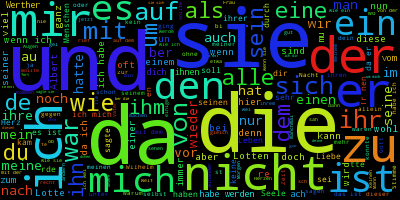
\includegraphics[width=1\textwidth]{res/beispielbild.png}
  \caption{Beispielbild \citep[nach][]{beispielbild}}
  \label{fig:exintink}
\end{figure}
Hello, here is some text without a meaning. This text should show what a printed text will look like at this place. If you read this text, you will get no information. Really? Is there no information? Is there a difference between this text and some nonsense like “Huardest gefburn”? Kjift – not at all! A blind text like this gives you information about \citep[nach][]{kreidenweis} the selected font, how the letters are written and an impression of the look. This text should contain all letters of the alphabet and it should be written in of the original language. There is no need for special content, but the length of words should match the language.

\subsection{Abschnitt 2.1}\label{Abschnitt21}
Hello, here is some text without a meaning. This text should show what a printed text will look like at this place. If you read this text, you will get no information. Really? Is there no information? Is there a difference between this text and some nonsense like “Huardest gefburn”? Kjift – not at all! A blind text like this gives you information about the selected font, how the letters are written and an impression of the look. This text should contain all letters of the alphabet and it should be written in of the original language. There is no need for special content, but the length of words should match the language.

\subsubsection{Abschnitt 2.1.1}\label{Abschnitt211}
Hello, here is some text without a meaning. This text should show what a printed text will look like at this place. If you read this text, you will get no information. Really? Is there no information? Is there a difference between this text and some nonsense like “Huardest gefburn”? Kjift – not at all! A blind text like this gives you information about the selected font, how the letters are written and an impression of the look. This text should contain all letters of the alphabet and it should be written in of the original language. There is no need for special content, but the length of words should match the language.

\subsubsection{Abschnitt 2.1.2}\label{Abschnitt212}
Hello, here is some text without a meaning. This text should show what a printed text will look like at this place. If you read this text, you will get no information. Really? Is there no information? Is there a difference between this text and some nonsense like “Huardest gefburn”? Kjift – not at all! A blind text like this gives you information about the selected font, how the letters are written and an impression of the look. This text should contain all letters of the alphabet and it should be written in of the original language. There is no need for special content, but the length of words should match the language.

% Seitenumbruch
\newpage

\section{Abschnitt 3}\label{Abschnitt3}
Hello, here is some text without a meaning. This text should show what a printed text will look like at this place. If you read this text, you will get no information. Really? Is there no information? Is there a difference between this text and some nonsense like “Huardest gefburn”? Kjift – not at all! A blind text like this gives you information about the selected font, how the letters are written and an impression of the look. This text should contain all letters of the alphabet and it should be written in of the original language. There is no need for special content, but the length of words should match the language.

\subsection{Abschnitt 3.1}\label{Abschnitt31}
Hello, here is some text without a meaning. This text should show what a printed text will look like at this place. If you read this text, you will get no information. Really? Is there no information? Is there a difference between this text and some nonsense like “Huardest gefburn”? Kjift – not at all! A blind text like this gives you information about the selected font, how the letters are written and an impression of the look. This text should contain all letters of the alphabet and it should be written in of the original language. There is no need for special content, but the length of words should match the language.

\subsection{Abschnitt 3.2}\label{Abschnitt32}
Hello, here is some text without a meaning. This text should show what a printed text will look like at this place. If you read this text, you will get no information. Really? Is there no information? Is there a difference between this text and some nonsense like “Huardest gefburn”? Kjift – not at all! A blind text like this gives you information about the selected font, how the letters are written and an impression of the look. This text should contain all letters of the alphabet and it should be written in of the original language. There is no need for special content, but the length of words should match the language.

\subsubsection{Abschnitt 3.3}\label{Abschnitt33}
Hello, here is some text without a meaning. This text should show what a printed text will look like at this place. If you read this text, you will get no information. Really? Is there no information? Is there a difference between this text and some nonsense like “Huardest gefburn”? Kjift – not at all! A blind text like this gives you information about the selected font, how the letters are written and an impression of the look. This text should contain all letters of the alphabet and it should be written in of the original language. There is no need for special content, but the length of words should match the language.

\subsubsection{Abschnitt 3.4}\label{Abschnitt34}
Hello, here is some text without a meaning. This text should show what a printed text will look like at this place. If you read this text, you will get no information. Really? Is there no information? Is there a difference between this text and some nonsense like “Huardest gefburn”? Kjift – not at all! A blind text like this gives you information about the selected font, how the letters are written and an impression of the look. This text should contain all letters of the alphabet and it should be written in of the original language. There is no need for special content, but the length of words should match the language.

\newpage

\section{Fazit}\label{Fazit}
Hello, here is some text without a meaning. This text should show what a printed text will look like at this place. If you read this text, you will get no information. Really? Is there no information? Is there a difference between this text and some nonsense like “Huardest gefburn”? Kjift – not at all! A blind text like this gives you information about the selected font, how the letters are written and an impression of the look. This text should contain all letters of the alphabet and it should be written in of the original language. There is no need for special content, but the length of words should match the language.


%\label{sec:refUeb2}
%Hier steht der Inhalt des zweiten Abschnitts
%Hier ein literaturverweis. Literatur muss in literatur.bib vorhanden sein \citep[vgl.][23]{beispiel2017}

%Hier der Inhalt von Überschrift 2 mit einem Beispielbild // und \citep[nach][12\psq]{ley2004soz} einem Literaturverweis
%\begin{figure}[hbtp]
%  \centering
%  
\includegraphics[width=0.85\textwidth]{res/hs_fulda_logo.png}
%  \caption{Exklusion - Integration - Inklusion \citep[nach][]{unbrk2009inklusion}}
%  \label{fig:exintink}
%\end{figure}
% label brauch man für verlinkungen, also in diesem fall unnötig
%\label{sec:refUeb1}

